\mychapter{4}{RSA and Integer Factorisation}
\begin{center}
	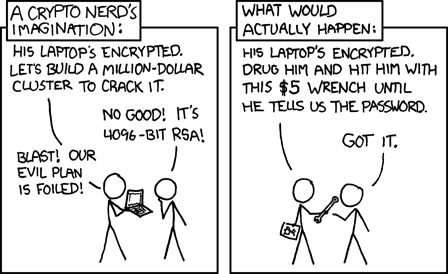
\includegraphics[width=0.75\textwidth]{Photos/RSA.png}
\end{center}

	\mysection{1}{What we have covered until now}
		We studied the Diffie Hellman and other cryptosystems based on the Discrete Logarithm Problem. Till now we have studied Fermat's Little Theorem, \[a^{p-1}\equiv 1 \bmod(p)\]
		Let us now try to generalise it for some composite number \(N\).
		
		\subsection{Euler's Formula}\label{subsec:EuclidFormula}
			If \(N = p \cdot q\), where \(p, q \in \text{primes}\), then we can write that \[a^{(p-1)(q-1)} \equiv 1 \bmod(p\cdot q) \equiv 1\bmod(N)\]Moreover, if \(g = \gcd(p-1,q-1)\), we can even write, \[a^\frac{(p-1)(q-1)}g \equiv 1 \bmod(p\cdot q) \equiv 1\bmod(N)\]
			\begin{tcolorbox}[title=Proof]
					Firstly, let us prove \(a^\frac{(p-1)(q-1)}g \equiv 1 \bmod(p)\) and \(a^\frac{(p-1)(q-1)}g \equiv 1 \bmod(q)\) separately. \par
					Because of the fact that both \(\frac pg\) and \(\frac qg\) are integers and using the Fermat's Little Theorem, we can trivially prove these to be true.\par
					Since both the equations are true, we can be sure that \(q\; |\;a^\frac{(p-1)(q-1)}g -1\) and \(p\; |\; a^\frac{(p-1)(q-1)}g-1\: \Rightarrow p\cdot q | a^\frac{(p-1)(q-1)}g-1\) since \(\gcd(p,q)=1\).
			\end{tcolorbox}

			Since we know that \(a^{(p-1)\cdot(q-1)}\equiv 1 \bmod(p\cdot q)\), we can write that any exponent \(x\) in the form \(a^x \equiv 1 \bmod(p\cdot q)\) lies in the ring \(\mathbb{Z}/\big((p-1)\cdot (q-1)\big)\mathbb{Z}\) and hence modulo \((p-1) \cdot (q-1)\) since $x=x$ gives the same results as $x=x+(p-1)\cdot (q-1)$.\par
			Actually, we infact, can write it exists in modulo \(\frac{(p-1)\cdot(q-1)}g\) because of the above formula.

	\mysection{2}{Integer Factorisation Problem}
		Now let us set the foundations for the RSA cryptosystem which depends on the integer factorisation problem. Until now, we have seen systems where DLP is used which asks you to solve for \(x\) when \(a, b \) and \(p\) and given in the following system- \[a^x \equiv b \bmod(p)\] Now we will deal with systems where security depends on the difficulty in finding \(x\) when \(e, c\) and \(N\) are known publicly- \[x^e \equiv c \bmod(N)\]
		
		\subsection{Is it really hard to find the \(e\)th root modulo \(N\)?}
			\subsubsection{\(N\in\text{primes}\)}
				Assume \(N = p \in \text{primes}\). In that case, finding the $e$th root is actually trivially easy. 
				\begin{mybox}
					If \(N = p\), we just need to solve for $d$ in \[d\cdot e\equiv 1 \bmod(p-1)\]\textbf{Reason?} We had discussed while studying the \hyperref[sec:pohlig]{Pohlig-Hellman Algorithm} that in \(a^x \equiv 1 \bmod(p)\), \(x\) belongs to the ring \(\mathbb{Z}/(p-1)\mathbb{Z}\) hence all calculations relating to it exist in modulo \((p-1)\) space.\par
					From the \hyperref[theo:extendedEuclid]{Extended Euclidean Theorem}, we know that finding \(d\) in the above congruence takes \textcolor{red}{linear time} \(\rightarrow\) trivially easy.\par
					After that we just need to calculate \(c^d \bmod(p)\) as \[x^e\equiv c \bmod(p)\Rightarrow(x^e)^d\equiv c^d \bmod(p)\Rightarrow x^1\equiv c^d \bmod(p)\] 
					\textbf{Note-} We need to choose \(e\) and \(p\) such that \(\gcd(e, p-1)=1\), else \(d\equiv e^{-1}\bmod(p-1)\) won't exist. 
				\end{mybox}

			\subsubsection{\(N\in\text{product of 2 primes}\)}	
				Let us now solve for \(N = p \cdot q\), where \(p, q \in \text{primes}\)-\par
				\[x^e\equiv 1\bmod(p\cdot q)\]
				Now we have to find the inverse \(d\) of \(e\) such that, \[x^{d\cdot e}\equiv x^1\equiv c^d\bmod(p\cdot q)\]To do that, we refer to \hyperref[subsec:EuclidFormula]{Euclid's formula}, to state that $d$ would satisfy \[d\cdot e \equiv 1 \bmod\big((p-1)\cdot (q-1)\big)\]Actually, to make our calculations easier henceforth (i.e. to get a smaller value of $d$), we use- \[d\cdot e \equiv 1 \bmod\bigg(\frac{(p-1)\cdot (q-1)}g\bigg)\]
				Solving for \(d\) in this is also very easy since \(\frac{\big((p-1)\cdot (q-1)\big)}{g}\) is a composite number which we can solve\footnote{Of course, $d$ will only exist if $\gcd(e, \big((p-1)\cdot (q-1)\big)/g)=1$} by finding the prime factors and then evaluating \(e^{-1}\) in each one of them and then weaving them together with \hyperref[subsec:chinese]{CRT}; all in \textcolor{red}{linear time}.

		\subsection{Then how is this cryptosystem even safe?}
			As of now, we have seen that if we can find the prime factors of any number \(N\), we can easily find the inverse \(d\) such that \(x \equiv c^d\). Finding individual inverses modulo primes takes linear time which calculating \(c^d\) takes \(\mathcal{O}(\log d)\) time. So how exactly can we say that this can be used to create a secure cryptosystem?\par
			Well the difficulty actually lies in the factorisation of \(N\) itself. The only way to find the inverse of \(e\), is by factorising \(N\) which becomes increasingly difficult as \(N\) increases. \\
			\textbf{Why?} We need to find \((p-1)\cdot (q-1)\) which is \(p \cdot q - (p + q) + 1= N - (p+q) +1\). Hence the only way to know \((p-1) \cdot (q-1)\) is if you know $p+q$ which means you know both $p$ and $q$ individually\footnote{There is some concern that this might not be completely true. Although \href{https://link.springer.com/content/pdf/10.1007/BFb0054117.pdf}{this paper}, states that ``an oracle for breaking RSA does not help in factoring integers'' but they couldn't prove any weakness in RSA because of that.} (by the quadratic formula).

	\mysection{3}{RSA Implementation}
		Named after the inventors (Rivest, Shamir, Adleman), RSA depends on the Integer Factorisation problem.
		\begin{itemize}
			\item \emph{Bob}\(\Rightarrow\)Chooses a $p,q\in \text{primes}$ to construct \(N= p \cdot q\). \(e\) is then selected such that \(\gcd(e, (p-1)\cdot (q-1))=1\)\footnote{There are some more nuances in selecting \(e\) which are discussed \hyperref[subsec:nuances]{later}.}
			\item \emph{Alice}\(\Rightarrow\)Converts her plaintext to an integer \(m\) such that \(1\leq m<N\). She then sends \(c \equiv m^e \bmod(N)\) to \emph{Bob.}
			\item \emph{Bob}\(\Rightarrow\)Finds \(d\) using \(d\cdot e \equiv 1 \bmod\big((p-1)\cdot (q-1)\big)\) and calculates \(c^d \equiv m^{e\cdot d}\equiv m \bmod(N)\).
			\item \emph{Eve}$\Rightarrow$This whole while had $m^e$ but inversion required her to factor \(N\) which is a difficult task without an easy algorithm as is the case with DLP.
		\end{itemize}

		\subsection{Nuances in choosing \(e\)}\label{subsec:nuances}
			Keep in mind that choosing \(e\) and \(d\) actually decides the time it takes for encryption and decryption respectively. In general, choosing a small \(e\) gives you a large \(d\), and vice versa (unless of course you go for \(e=d=1\)).
			\begin{itemize}
				\item We can choose a small \(e\;\Rightarrow\) large $d\Rrightarrow$ Ensures faster encryption, but slower decryption.\\
				\(\rightarrow\)There is some concern that a small $e$ might cause issues so a lot of people prefer to use $e=2^{16}+1$\footnote{Although this looks like a huge exponent for calculating $m$, it is just 4 squarings and 1 addition}. But there is no evidence that \(e=3\)\footnote{We cannot use $e=2$ since \(\gcd(p-1,q-1)\) for large $p,q$ will be $2$.} is any less secure than a larger $e$.
				\item We can choose a small \(d\; \Rightarrow\) large \(e\Rrightarrow\) Ensures faster decryption, but slower encryption.\\
				\(\rightarrow\)This is actually \textcolor{red}{extremely insecure} as \(d<N^\frac14\) can be easily decrypted using theory of continued fractions.
			\end{itemize}

			It is not compulsory for \emph{Eve} to factor \(N\) to solve a RSA cryptosystem but at the same time, we have yet not found any such alternative method. (Like how we found \hyperref[sec:colli]{Collision Algorithms} in DHP)

		\subsection{Security issues in RSA}	
			Just like in DHP, there exist some security concerns with the RSA system which can just circumvent having to solve the underlying problem. 

			\begin{tcolorbox}[title=RSA Oracle Method, breakable, colback=yellow!5!white,colframe=yellow!75!black]
 			\emph{Eve} asks \emph{Alice} to authenticate her identity by sending her messages encrypted using the public \(e, N\) she has put up and asking her to tell her the decrypted/original message. This request makes some practical sense as it is feasible for \emph{Eve} to be talking to someone who isn't \emph{Alice} in which case this impostor won't be able to send her back the original text\footnote{By original message, we obviously mean \emph{Alice} is expected to send \emph{Eve} whatever she decrypted with her private key and then encrypt it with \emph{Eve'}s public key as that is standard practice.}\vspace{0.5cm}
 			If \emph{Alice} decides to do so and sends back whatever gibberish she gets after decryption for a few messages, \emph{Eve} can easily employ the following method to decrypt \emph{Bob'}s messages that were meant for \emph{Alice} but intercepted by \emph{Eve}.\vspace{0.5cm}
 			\emph{Bob} enrypts messages \(m\) as \(m'\equiv m^e \bmod(N)\) and \emph{Eve} gets her hands on it. \emph{Eve} then compute \(m''\equiv k^e \cdot m' \bmod(M)\) where \(k\in \text{random constant}\) and send $m''$ to \emph{Alice.} \vspace{0.5cm}
 			She returns back \((m'')^{d}\equiv k\cdot m \bmod(N)\). Since \(k\cdot m\) will be gibberish, \emph{Alice} cannot read the original message and \emph{Eve} can easily just get back \(m\).
 			\tcblower
 			A good practice that \emph{Alice} can follow to not fall prey to such attacks is to not send back decrypted messages to any person for authentication purposes if they don't follow a specific format; especially if they are gibberish. 
		\end{tcolorbox}

		\begin{tcolorbox}[title=Multiple encryption exponents for the same modulo, breakable, colback=yellow!5!white,colframe=yellow!75!black]
 			If \emph{Alice} decided to keep different keys for different sets of people in her online life, she can do that by changing both $N$ and $e$ or by just changing \(e\) for the same \(N\). The second method is fatal to the security of her system though.\\
 			\textbf{How?}\vspace{0.5cm}
 			Let's say that the 2 exponents are \(e_1\) and \(e_2\). If somehow, there comes a situation wherein \emph{Eve} intercepts 2 ciphers \(c_1\) and \(c_2\) of the same message \(m\), she can write\footnote{Using the \hyperref[subsec:gcd]{property of gcd}}-
 			\[u\cdot e_1 + v \cdot e_2 = \gcd(e_1, e_2)\]
 			After finding suitable \(u\) and \(v\), she can compute-
 			\[c_1^u \cdot c_2^v \equiv m^{e_1\cdot u + e_2 \cdot v}\equiv m^{\gcd(e_1,e_2)} \bmod(N)\]
 			If $e_1$ and $e_2$ are relatively prime, we can directly find the plaintext \(m\).\vspace{0.5cm}
 			Note that if \(\gcd(e_1, e_2)\not = 1\), we still have to solve \(x^\alpha\equiv h \bmod(N)\) which is pretty difficult even if \(\alpha \ll e_1, e_2\)\footnote{As was discussed earlier, there is no evidence $e=3$ is any easier to solve than a larger \(e\).}. 
 			\tcblower
 			Although this method requires a lot of things to line up (\emph{Bob} verifiably sending the same message via 2 exponents, \(e_1\) and \(e_2\) being coprime), it is a weakness that \emph{can} manifest unknowingly if \emph{Alice} decided to make even more keys. Hence it is good practice to use a different modulo for every key. 
		\end{tcolorbox}

	\mysection{4}{Primality testing}
		Before \emph{Bob} can begin communication with anyone in the RSA system, he has to choose a \(p, q\in \text{very very large primes}\). \\
		\begin{itemize}
			\item If he goes for small primes, today's computers can easily factorise $N$.
			\item If either one of $p$ and $q$ ends up as composite with small prime factors, \emph{Eve} can easily work with CRT to bring down the system's security. 
			\item If either one of $p$ and $q$ is composite with large prime factors, \emph{Bob} will have to spend computation time in trying to find the factors else he won't be able to decrypt \emph{Alice's} messages.
		\end{itemize}
		Now for us to satisfy all of these conditions, \emph{Bob} first will choose a fairly large number and then check if it is prime and, if not, do the same with the next number until he finds a prime.\\
		But once he has a number, how can he verify that it is prime?
		\begin{itemize}
			\item[\(\star\)] The first idea that can come to mind is to naively check if all numbers from 2 to \(\sqrt{n}\) are coprime with $n$.\\This however is \(\mathcal{O}(\sqrt{n})\Rightarrow\) \textcolor{red}{Exponential time}.
		\end{itemize}
		\subsection{Fermat Primality test}
			So we go with exploiting \hyperref[sec:fermat]{Fermat's Little Theorem}\footnote{We will use a slightly different version. Fermat's ``Little'' theorem states that for \(a\nmid p\text{, }a^{p-1}\equiv 1 \bmod(p)\). This puts a restrictions which can be lifted by instead denoting it as \(a^p \equiv a \bmod(p)\).}. We know that for every prime number \(p\), \[a^p \equiv a \bmod(p)\]This is \textbf{not compulsorily} false for composite numbers. \\e.g. \(2^{341}\equiv 2 \bmod(341)\) although \(341 = 11 \cdot 31\). \par
			We then define the concept of ``witnesses''.

			\subsubsection{Witnesses}\label{subsec:witness}
				\begin{mybox}
					For a number \(n\), any \(a\) such that \[a^n \not \equiv a \bmod(n)\] is called the ``\textcolor{red}{witness}'' of \(n\).
				\end{mybox}	
				After checking a large number of candidates \(\{k_1, k_2, k_3, \ldots, k_l\}\), if we cannot find a witness for \(n\), we can be reasonably sure that \(n\) is prime; but we cannot be 100\% certain.\par
				Keep in mind that there exists a subset of numbers called \textcolor{red}{Carmicheal Numbers} which do not have any witnesses despite being composite. e.g. 561\\
				There exist \(\infty\)ly many such numbers and hence, even if you couldn't find a single witness, it doesn't prove primality.

		\subsection{Miller-Rabin test for Primality}
			The Miller-Rabin test depends on the following propostion.

			\begin{tcolorbox}[title=Proposition, breakable]
				If \(p\in \text{odd primes}\), and we write \(p= 2^k \cdot q + 1\), where \(q\in \text{odd integers}\), we can say that the following it will satisfy either of the 2 following properties-
				\begin{enumerate}
					\item \(a^q\equiv 1 \bmod(p)\) \[\text{OR}\]
					\item One element in the series \(a^q, a^{2q}, a^{4q}, \ldots, a^{2^{k-1}q} \bmod(p)\) is congruent to \(-1\). 
				\end{enumerate}
			\end{tcolorbox}

			\begin{tcolorbox}[breakable, title=Proof,colback=red!5!white,colframe=red!75!black]
				Consider \(a^{q\cdot 2^{k}}\bmod(p)\). It is obviously equivalent to \(a^{p-1}\equiv 1 \bmod(p)\). Also all of the terms in the series \(a^q, a^{2q}, a^{4q}, \ldots, a^{2^{k}q} \bmod(p)\) are actually in series of squares so if the last term is 1, the only possibility is that \(a^{q\cdot 2^{k-1}}\equiv \pm 1 \bmod(p)\). 

				\begin{itemize}
					\item If \(a^{q\cdot 2^{k-1}}\equiv - 1 \bmod(p)\), condition \textcolor{orange}{2} is satisfied.
					\item If \(a^{q\cdot 2^{k-1}}\equiv + 1 \bmod(p)\), \(a^{q\cdot 2^{k-2}}\equiv \pm 1 \bmod(p)\) \small
						\begin{itemize}
							\item If \(a^{q\cdot 2^{k-2}}\equiv - 1 \bmod(p)\), condition \textcolor{orange}{2} is satisfied.
							\item If \(a^{q\cdot 2^{k-2}}\equiv + 1 \bmod(p)\), \(a^{q\cdot 2^{k-3}}\equiv \pm 1 \bmod(p)\) \scriptsize
								\begin{itemize}
									\item If \(a^{q\cdot 2^{k-3}}\equiv - 1 \bmod(p)\), condition \textcolor{orange}{2} is satisfied.
									\item If \(a^{q\cdot 2^{k-3}}\equiv + 1 \bmod(p)\), \(a^{q\cdot 2^{k-4}}\equiv \pm 1 \bmod(p)\)\\
										\textcolor{orange}{\[\vdots\]}\normalsize
										\[\quad \quad \quad a^q\equiv 1 \bmod(p)\text{ and thus condition \textcolor{orange}{1} is satisfied.}\]
								\end{itemize}
						\end{itemize}
				\end{itemize}

			\end{tcolorbox}

			Now let us develop the algorithm for using this primality test.

			\subsubsection{Miller-Rabin witnesses}
			A \textcolor{red}{Miller-Rabin witness} ($a$) will satisfy BOTH the following 2 conditions-
			\begin{enumerate}
				\item \(a^q\not \equiv 1\bmod(p)\)
				\item \(a^{q\cdot 2^i}\not \equiv -1 \bmod(p)\quad \forall i\in [0,k-1]\)
			\end{enumerate}

			\begin{tcolorbox}[title=Digesting the meaning of witness here]
				We know from Fermat's primality test, that if \(a^{p-1}\equiv 1 \bmod(p)\), then \(p\) is probably a prime number. So if either one of the 2 congruences was true, obviously \(p\rightarrow \text{probably prime}\). \par

				Hence the definition of a Miller-Rabin Witness means that if the 2 properties are followed (i.e. both congruences are false), the number \(p\) is \textcolor{red}{definitely composite}.
			\end{tcolorbox}

			\underline{\textbf{Algorithm for Miller-Rabin test}}
			\begin{enumerate}
				\item To check \(n\)'s primality, choose a value of \(2\leq a\leq n-1 \) (candidate for a witness) and find \(q\) and \(k\) such that, \[n=2^k\cdot q +1\] 
				\item Evaluate values of \(a^q, a^{2\cdot q}, a^{4\cdot q},\ldots, a^{2^{k-1}\cdot q} \bmod(p)\) (use fast exponentiation) and check if \(a\) is a valid Miller-Rabin witness.
				\item If \(a\)-
					\begin{enumerate}
						\item is a witness- \(n\) is definitely composite
						\item is not a witness- \(n\) is probably prime. If so, choose another value of \(a\) and try again for better resolution. 
					\end{enumerate}
			\end{enumerate}

			\Large \centering{\textcolor{orange}{But what makes Miller-Rabin test better than Fermat test?}}

			\normalsize\raggedright \textcolor{red}{At least 75\% of the bases from \(2\) to \(n-1\) are Miller-Rabin witnesses if \(n\in\) composite.} Hence even Carmicheal numbers get caught by this algorithm even though Fermat cannot find even a single witness for them. \\So if you chose 10 bases and got not a single Miller-Rabin witness, the probabilty of it not being a prime number is \((0.25)^{10}\approx9.54\times 10^{-7}\). (If there are 0 witnesses in 100 bases selected, probability of it being composite\(=10^{-60}\))

			\begin{mybox}
				One interesting fact is that \textbf{every} composite number has a \(\frac14\) chance of passing the Miller-Rabin test as a ``probably prime number'' for a specific base.\\
				Fermat primality test has the same statistics for \textbf{ever non-Carmicheal} composite number.
			\end{mybox}

			\begin{tcolorbox}[breakable, title=Illustration,colback=brown!5!white,colframe=brown!75!black,colbacktitle=yellow!50!red,coltitle=red!25!black,fonttitle=\bfseries,subtitle style={boxrule=0.4pt,colback=yellow!50!red!25!white} ]
				Check if \(n= 172947529\) is prime or not\vspace{0.5cm}
				\hrule
				\vspace{0.5cm}
				\[n-1=172947528=2^3\cdot21618441\quad\rightarrow\quad k=3\text{ and }q=21618441\]
				Choose \(a=3\Rrightarrow\)
				\[3^{21618441}\equiv -1 \bmod(172947529)\]
				So \(a=3\) is not a witness.

				Let us try $a=17$-
				\[17^{21618441}\equiv 1 \bmod(172947529)\]
				Again not a witness. We might suspect that 172947529 might actually just be a prime.

				But on further analysis with \(a=23\), we get-
				\[23^{21618441}\equiv40063806\bmod(172947529)\]
				\[23^{2\cdot 21618441}\equiv 2257065\bmod(172947529)\]
				\[23^{4\cdot 21618441}\equiv 1\bmod(172947529)\]
				In this whole sequence, not once did we get congruence of \(-1\) and the first term was not congruent to $1$. Hence $23$ is actually a witness of $172947529$.\par
				\textbf{But wait.} \\~\\ \textcolor{brown}{Isn't \(23^{8\cdot 21618441}\equiv 2257065\bmod(172947529)\) here?}\\Yes.\\~\\\textcolor{brown}{Doesn't that mean that it is ``probably prime'' according to Fermat primality?}\\Yes. But that is irrelevant. \\\textbf{All} prime numbers don't have either witnesses but \textbf{some} composite numbers would give a ``false-positive'' with Fermat but not so with Miller-Rabin.

			\end{tcolorbox}

	\mysection{5}{Factorisation algorithm}
		Till now we have discussed how we need to choose large \(p,q\) while constructing \(N\) and also discussed a bit about how to choose large primes without wasting too much computation in deternmining if it is prime or not. Yet, choosing large primes, despite all the optimisations, remains a computationally heavy task. In that case, it is of significant use to understand the algorithms that \emph{Eve} can use to factorise $N$ and try to optimise our order of $p,q$ in accordance.\\~\\
		The easiest algorithm we can study is the Pollard's \(p-1\) factorisation algorithm.

		\subsection{Pollard's \(p-1\) factorisation algorithm}
			Let $N=p\cdot q \quad p,q\in$ primes. 
			\begin{itemize}
				\item Assume for a second that you can choose a $L$ such that \((p-1) | L\) but \((q-1) \nmid L\).
				\item Then we can write that \(a^{p-1}\equiv 1 \bmod(p) \Rightarrow a^L\equiv 1 \bmod(p)\).
				\item Thus we can say that \(p | (a^L-1)\) but at the same time \(q \nmid (a^L-1)\).
				\item Since \(p\in\) primes, obviously \[p=\gcd(a^L-1, N)\]
			\end{itemize}

			\textbf{But how do you find this famed \(L\)?}\\
			Well you can take the reasonable assumption that $(p-1)$ has a lot of small prime factors. In that case, if we chose a random large \(n\), we can expect \(p-1 | n!\) thus we can take \(L= n!\). 

			Now obviously, the roots of $(q-1)$ are also allowed to exist in $n!$ by happenstance so in the case that $(q-1)\cdot (p-1) | n!$, we might get \(\gcd(a^{n!}-1, N)=N\)\footnote{Essentially $a^{n!}\equiv1\bmod(p)$ and $a^{n!}\equiv1\bmod(q)$ would be both true simultaneously hence $a^{n!}\equiv1\bmod(p\cdot q)\equiv 1 \bmod(N)$} which is completely useless. \par So we will definitely have to vary $n!$ a little bit in the hopes that only one of $p-1$ or $q-1$ is completely able to divide $n!$. But there is a good chance that it will be useless. So in that case, we just vary $a$\footnote{How does this change $\gcd$ in any meaningful way?\\Essentially we can write \(a^{n_1!}-1 = \kappa_1 (p-1)\cdot (q-1)\). But if we changed $n_1$ to $n_2$, since there is a chance the primes factors of both $(p-1)$ and $(q-1)$ are still both present in $n_2!$ i.e. \(a^{n_2!}-1 = \kappa_2 (p-1)\cdot (q-1)\)\\However if we changed \(a_1\) to \(a_2\), it might be possible that $(q-1) | a_2$ in which case $a_2^{n!}\equiv 0\bmod(q)$ hence $a_2^{n!}-1$ is just a multiple of $(p-1)$}.\par

			\begin{tcolorbox}
				You might be worried that you will have to evaluate gcd of $N$ and a larger number \(a^{n!}-1\) but you can actually use Euclid's algorithm for gcd and then find the gcd(\(N, a^{n!}-1 \bmod(p)\)). Yay!
			\end{tcolorbox}


